\documentclass[10pt, a4paper]{report}

\usepackage[utf8]{inputenc}
\usepackage{polski}
\usepackage{a4wide}
\usepackage{fancyhdr}
\usepackage{lastpage}
\usepackage{tabularx}
\usepackage{graphicx}
\usepackage{listings}
\usepackage{forest}
\usepackage{xcolor}


\graphicspath{ {./images} }

\definecolor{folderbg}{RGB}{124,166,198}
\definecolor{folderborder}{RGB}{110,144,169}
\definecolor{codegreen}{rgb}{0,0.6,0}
\definecolor{codegray}{rgb}{0.5,0.5,0.5}
\definecolor{codepurple}{rgb}{0.58,0,0.82}
\definecolor{backcolour}{rgb}{0.95,0.95,0.92}

\lstdefinestyle{listings}{
    backgroundcolor=\color{backcolour},   
    commentstyle=\color{codegreen},
    keywordstyle=\color{magenta},
    numberstyle=\tiny\color{codegray},
    stringstyle=\color{codepurple},
    basicstyle=\ttfamily\footnotesize,
    breakatwhitespace=false,         
    breaklines=true,                 
    captionpos=b,
    keepspaces=true,                 
    numbers=left,                    
    numbersep=6pt,                  
    showspaces=false,                
    showstringspaces=false,
    showtabs=false,                  
    tabsize=4
}

\def\Size{4pt}
\tikzset{
  folder/.pic={
    \filldraw[draw=folderborder,top color=folderbg!50,bottom color=folderbg]
      (-1.05*\Size,0.2\Size+5pt) rectangle ++(.75*\Size,-0.2\Size-5pt);  
    \filldraw[draw=folderborder,top color=folderbg!50,bottom color=folderbg]
      (-1.15*\Size,-\Size) rectangle (1.15*\Size,\Size);
  }
}

\begin{titlepage}
    \title{\huge{\textbf{Sprawozdanie} \\ programu grapher}}
    \author{Szymon Półtorak i Sebastian Sikorski}
    \date{14.04.2022r}
\end{titlepage}

\renewcommand{\footrulewidth}{1pt}
\lstset{style=listings}

\begin{document}
    \maketitle

    \renewcommand*\thesection{\arabic{section}}
    
    \begin{abstract}
        Niniejszy dokument jest sprawozdaniem z prac projektowych w ramach projektu \textit{grapher} w języku C.
        W dokumencie został przypomniany cel projektu, opisana struktura folderów, diagram modułów, przedstawione
        wywołania programu wraz z ich wynikami. Podsumowaliśmy projekt oraz współpracę i wysnuliśmy wnioski na temat tego przedsięwzięcia.
    \end{abstract}

    \pagestyle{fancy}
    \fancyhf{}
    \lhead{Sprawozdanie programu \textit{grapher}(C)}
    \rhead{Szymon Półtorak i Sebastian Sikorski}
    \cfoot{Strona \thepage \hspace{1pt} z \pageref{LastPage}}
    
    \fancypagestyle{plain}{
        \lhead{Sprawozdanie programu \textit{grapher}(C)}
        \rhead{Szymon Półtorak i Sebastian Sikorski}
        \cfoot{Strona \thepage \hspace{1pt} z \pageref{LastPage}}
    }
    \tableofcontents
    \newpage

    \section{Cel projektu}
    Celem projektu było stworzenie programu mającego za zadanie generowanie grafów, sprawdzanie ich spójności oraz wyszukiwanie w nich najkrótszej ścieżki między zadanymi przez użytkownika punktami. 
    Grafi są typu \textit{kartka w kratkę}.

    \begin{itemize}
        \item Wage Mode – program generuje graf o losowych wagach dróg między wierzchołkami w taki sposób, że jest on spójny,
        \item Edge Mode – program losuje istnienie krawędzi między wierzchołkami grafu oraz wagi do momentu powstania 
        grafu spójnego. Do sprawdzania wykorzystuje algorytm BFS,
        \item Random Mode – program losuje wagi dróg oraz krawędzie między wierzchołkami. W tym trybie graf może być niespójny,
        \item Read Mode -- program odczytuje odpowiednio sformatowany plik i szuka najkrótszej ścieżki
        między podanymi przez użytkownika punktami za pomocą algorytmu Dijkstry. Format pliku zostanie opisany w osobnej podesekcji, sekcji trzeciej.
    \end{itemize}
    Struktura grafu oparta jest na koncepcji "kartka w kratkę" tzn. graf składa się z wierzchołków równo rozmieszczonych na liniach poziomych 
    i pionowych wyznaczanych przez liczbę wierszy i~ kolumn. Jedyne połączenia zachodzące między wierzchołkami dozwolone są  pionowo i poziomo co pokazuje poniższy diagram, na którym zostały zaznaczone jedynie wagi wybranych krawędzi aby zachować czytelność całego diagramu, jednocześnie obrazując schemat połączeń.
    \begin{figure}[ht]
        \begin{center}
            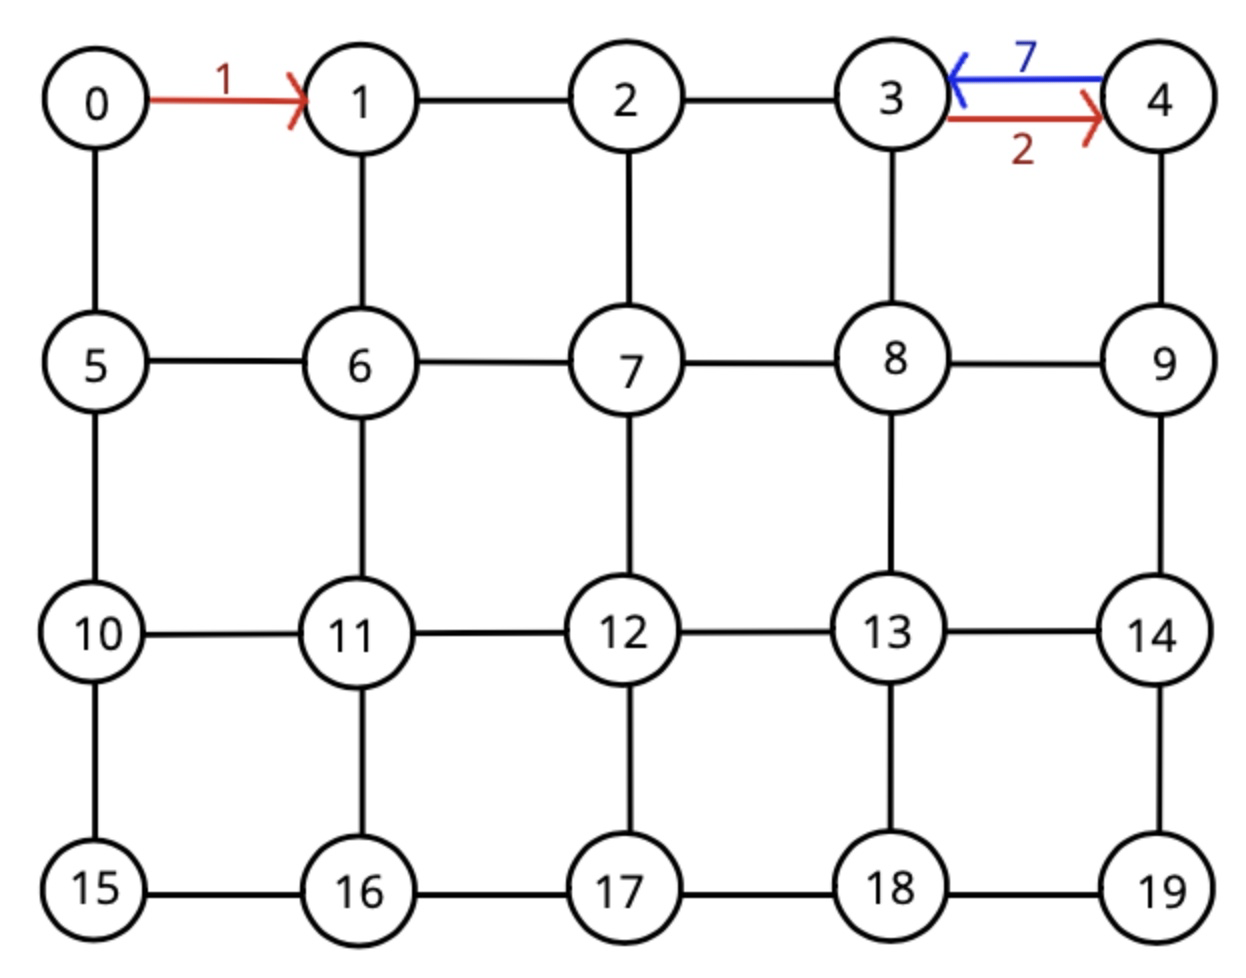
\includegraphics[scale=0.15]{graph.png}
            \caption{Przykład grafu typu "kartka w kratkę"}
        \end{center}
    \end{figure}

    \section{Struktura programu}
    Program \textit{grapher} skłąda się z 4 folderów nadrzędnych zawierających jego poszczególne elementu. Folder \textit{dokumentacja} zawiera dokumenty opisujące projekt, czyli:
    specyfikację funkcjonalną i implementacyjną oraz końcowe sprawozdania z projektu. Są w nich pliki \textit{*.pdf}, zdjęcia w formacie \textit{*.png} i \textit{*.jpg} oraz kod źródłowy tych dokumnetów w formacie
    \textit{*.tex}. Folder \textit{tests} zawiera kod odpowiedziany za przeprowadzanie testów programu, natomiast folder \textit{src} zawiera pliki z kodem źródłowym oraz pliki nagłówkowe
    programu \textit{grapher}.

    \subsection{Struktura folderów}  
    \begin{forest}
        for tree={
          font=\ttfamily,
          grow'=0,
          child anchor=west,
          parent anchor=south,
          anchor=west,
          calign=first,
          inner xsep=7pt,
          edge path={
            \noexpand\path [draw, \forestoption{edge}]
            (!u.south west) +(7.5pt,0) |- (.child anchor) pic {folder} \forestoption{edge label};
          },
          before typesetting nodes={
            if n=1
              {insert before={[,phantom]}}
              {}
          },
          fit=band,
          before computing xy={l=15pt},
        }  
        [\texttt{Grapher}
        [\texttt{dokumentacja}
            [\texttt{Specyfikacja Implementacyjna}
                [\texttt{images}]
            ]
            [\texttt{Specyfikacja Funkcjonalna}
            ]
            [\texttt{Sprawozdanie}
                [\texttt{images}]
                [\texttt{listing}]
            ]
        ]
        [\texttt{tests}
            [\texttt{data}]
        ]
        [\texttt{src}
        ]
        [\texttt{makefile}
        ]
      ]
    \end{forest}

    \subsection{Diagram modułów}
    Projekt \textit{grapher} składa się z modułów: \textit{alloc}, \textit{readGraph}, \textit{genGraph} oraz \textit{utils}. 
    Każdy moduł składa się z pliku nagłówkowego \textit{*.h} oraz pliku z kodem źródłowym \textit{*.c}.
    Posiada on również główny moduł \textit{main} sterujący działaniem całego programu i składa się on tylko z pliku źródłowego \textit{main.c}.
    \begin{figure}[ht]
        \begin{center}
            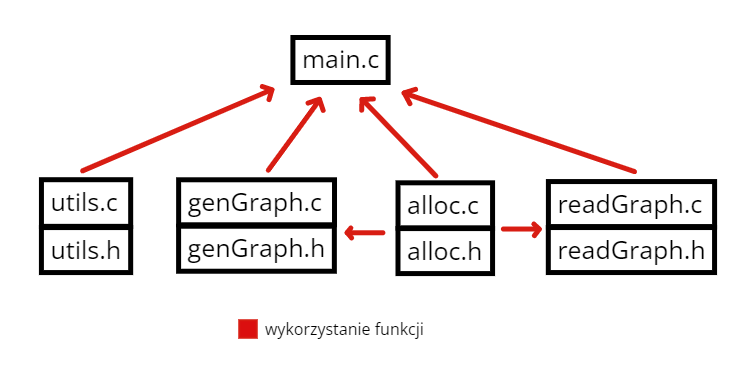
\includegraphics[scale=0.8]{module_diagram_new.png}
            \caption {Diagram modułów}
        \end{center}
    \end{figure}

    \section{Kompilacja programu}
    Program trzeba najpierw skompilować w katalogu głównym projektu. Poniżej przedstawiamy wszystkie komendy możliwe do użycia:
    \begin{itemize}
        \item \texttt{make} -- podstawowa kompilacja programu grapher,
        \item \texttt{make clean} -- usuwa z programu wszystkie pliki robocze oraz skompilowany plik do uruchamiania programu \textit{grapher},
        \item \texttt{make wm} -- kompiluje program i uruchamia go w trybie \textit{wage mode} z góry zakładanymi danymi,
        \item \texttt{make rem} -- robi to samo co powyższa komenda ale uruchamia program w trybie \textit{random mode},
        \item \texttt{make em} -- wykonuje to samo co powyższe 2 instrukcje ale uruchamia program w trybie \textit{edge mode},
        \item \texttt{make rm\_s} -- również wykonuje to samo zadanie ale program korzysta z trybu \textit{read mode} z flagą \textit{standard},
        \item \texttt{make rm\_e} -- działa indentycznie jak powyższa z tą różnicą, że z flagą \textit{extended}
        \item \texttt{make test} -- komenda służy do wykonania testów funkcji programu.
    \end{itemize}

    \section{Przykładowe wywołania i wyniki programu}
    W tym rozdziale przedstawimy wywołania programu wraz z ich wynikami dla różnych scenariuszów aby ukazać jak nasz program działa.

    \subsection{Plik wejściowy dla trybów generujących}
    W trybach generujących może to być plik pusty ale może to być również plik z danymi z tym, że zostanie on w całości nadpisany.

    \subsection{Wage Mode}
    Wywołanie:
    \newline\newline \texttt{./grapher -wm -rows 3 -start 1 -file tests/data/wg.test -end 10 -columns 3}
    \newline\newline Wynik:
    \lstinputlisting{listing/wg.txt}

    \subsection{Edge Mode}
    Wywołanie:
    \newline\newline \texttt{./grapher -em -rows 3 -file tests/data/em.test -end 20 -columns 4 -start 5}
    \newline\newline Wynik:    
    \lstinputlisting{listing/em.txt}

    \subsection{Random Mode}
    Wywołanie:
    \newline\newline \texttt{./grapher -rem -file tests/data/rem.test -end 10 -rows 4 -start 1 -columns 4}
    \newline\newline Wynik:
    \lstinputlisting{listing/rem.txt}
    \newpage

    \subsection{Read Mode z flagą Standard}
    \textbf{Plik wejściowy} :
    \lstinputlisting{listing/rm_s.txt}
    Wywołanie:
    \newline\newline \texttt{./grapher -rm -file tests/data/rm\_s.test -points 1,5,4,8 -standard }
    \newline\newline Wynik:
    \begin{figure}[ht]
        \begin{center}
            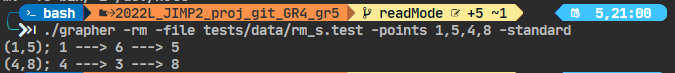
\includegraphics[scale=0.8]{rm_s.png}
            \caption {Wynik działania dla Read Mode z flagą -standard}
        \end{center}
    \end{figure}
    \newpage

    \subsection{Read Mode z flagą Extended}
    \textbf{Plik wejściowy} :
    \lstinputlisting{listing/rm_e.txt}
    Wywołanie:
    \newline\newline \texttt{./grapher -rm -extended -points 2,7,3,11 -file tests/data/rm\_e.test}
    \newline\newline Wynik:
    \begin{figure}[ht]
        \begin{center}
            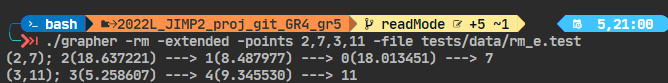
\includegraphics[scale=0.8]{rm_e.png}
            \caption {Wynik dla Read Mode z flagą -extended}
        \end{center}
    \end{figure}

    \newpage
    \section{Zmiany względem specyfikacji}
    W nieniejszym rozdziale opisujemy zmiany jakie zaszły między specyfikacją funkcjonalną i implementacyjną, a wersją finalną programu.

    \subsection{Diagram modułów}
    Z powodu potrzeby dodania nowego modułu zmienił się również diagram modułów.
    Doszedł moduł \textit{utils} wspomagający pracę \textit{maina} w zakresie obsługi błędów. Zostały dodane trzy nowe moduły \textit{tools}, \textit{options} oraz \textit{utils}. Ten pierwszy przechowuje funkcje odpowiedzialne za kolejkę oraz sprawdzanie spójności grafu, drugi
    wspomaga działanie \textit{maina} w taki sposób, że przejmuje jego odpowiedzialność w zakresie wywoływania funkcji odpowiadających za działanie trybów oraz za przypisywanie wartości z wywołania programu. Moduł \textit{utils} jest modułem współpracującym z \textit{options}.
    Pomaga on w sprawdzaniu danych wejściowych oraz weryfikuje podanie wszystkich niezbędnych wartości.
    Poniżej pokażemy starą wersję diagramu modułów, a wersja najnowsza jest przedstawiona wyżej.

    \begin{figure}[ht]
        \begin{center}
            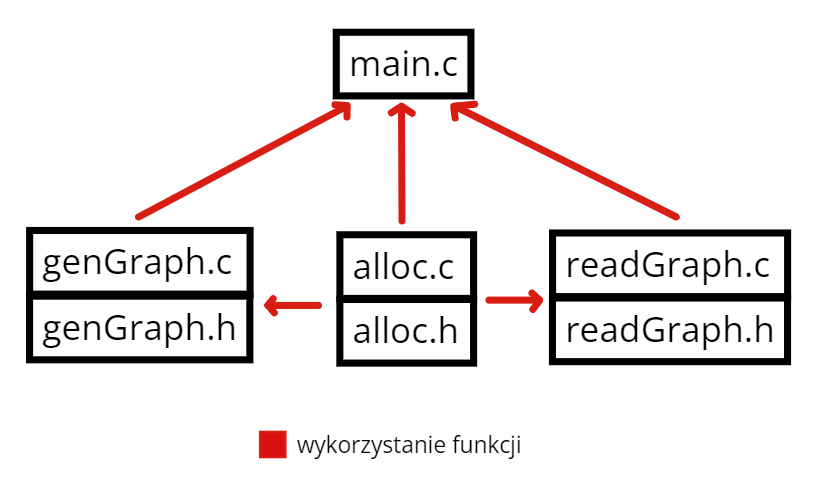
\includegraphics[scale=0.35]{module_diagram_old.jpg}
            \caption{Diagram modułów -- stara wersja}
        \end{center}
    \end{figure}

    \subsection{Obsługiwane błędy}
    W trakcie pisania programu napotkaliśmy na sytuacje, które wymagają zdefiniowania nowych błędów żeby użytkownik wiedział, dlaczego program się wyłączył.
    Niestety okazało się również, że nasze kody błędów były zbyt duże i program nie mógł zwracać takich wartości dlatego musieliśmy podjąć decyzję o ich zmianie.
    \newline Poniższa tabela zawiera wszystkie zadeklarowane błędy w programie:
    \newline
    \begin{tabularx}{\textwidth}{ l|c|X } 
        \hline Nazwa Błędu & Kod & Wyjaśnienie błędu\\ 
        \hline NO\_MODE\_FOUND & 226 & Niepoprawny tryb lub jego brak\\ 
        \hline NO\_FILE\_FOUND & 231 & Nie podano pliku lub plik nie istnieje\\ 
        \hline WRONG\_NUM\_OF\_ROWS & 232 & Podano niepoprawną liczbę wierszy\\
        \hline WRONG\_NUM\_OF\_COL & 233 & Podano niepoprawną liczbę kolumn\\
        \hline WRONG\_RANGE\_OF\_WAGES & 234 & Zły zakres losowania wartości wag\\
        \hline NO\_FLAG\_FOUND & 235 & Nie podany flagi w trybie Read Mode\\
        \hline WRONG\_POINTS & 228 & Podano nieistniejący punkt lub ich złą liczbę\\
        \hline NO\_COHERENT & 237 & Graf jest niespójny \\
        \hline NULL\_POINTER\_EXCEPTION & 228 & Alokacja pamięci się nie udała\\
        \hline NOT\_READ\_MODE & 229 & Użyto flagi w trybie do generacji, ale działającej tylko w Read Mode\\
        \hline MULTIPILE\_MODE\_DECLARATION & 230 & Dokonano próby nadpisania zadeklarowanego wcześniej trybu programu\\
        \hline WRONG\_MODE & 227 & Użyto flagi w trybie Read, ale działającej tylko w trybach generujących\\
        \hline INVALID\_DATA & 225 & Nie podano wymagano argumentu lub podano flagę, która nie istnieje\\
        \hline NO\_COL\_ROWS\_FOUND & 223 & W pliku do czytania nie znaleziono kolumn lub wierszy\\
        \hline NO\_NODES\_FOUND & 220 & W trybie nie znaleziono wierzchołków\\
        \hline
    \end{tabularx}

    \subsection{Zmiany w strukturach}
    Struktury również przeszły małe modyfikacje spowodowane nieprzewidzianymi potrzebami. Zaprezentujemy je poniżej.
    \begin{itemize}
        \item \texttt{struct entryRead} -- ta struktura otrzymała nową zmienną \textit{numberPoints} odpowiedzialną za przetrzymywanie liczby
        wszystkich punktów podanych przez użytkownika oraz zmieniliśmy typ zmiennej \textit{printFlag} żeby móc sprawdzać poprawnie jego podanie. Dodano również
        dwie nowe zmienne \textit{rows} i \textit{columns} odpowiedzialne za przechowanie liczby wierzchołków i kolumn,
        \lstinputlisting[language=C]{listing/entryRead.txt}
        \item \texttt{struct graphRead} -- została całkowicie usunięta, ponieważ podczas implementacji okazała się bezużyteczna,
        \item \texttt{struct node} -- ta struktura otrzymała nową zmienną tablicową \textit{nodeToConnect} oraz wszystkie tablice zostały zmienione ze wskaźników na tablice o określonym rozmiarze. 
        \lstinputlisting[language=C]{listing/node.txt}
    \end{itemize}

    \subsection{Wywoływanie programu}
    Zmianom uległo samo wywołanie programu. Poprzednio zakładaliśmy, że użytkownik będzie musiał przestrzegać kolejności wywołania, ale w czasie
    pisania programu stwierdziliśmy, że jest to zadanie bezsensowne i teraz użytkownik może wprowadzać przy pomocy odpowiednich flag w dowolnej kolejności poza jednym wyjątek. Owym wyjątkiem jest tryb działania
    programu, który musi być podawany jako pierwszy argument wywołania programu.
    Teraz flagi wymagają od użytkownika podania liczb po niektórych flagach. Poniżej przedstawiamy składnię programu.
    \newline Dla trybów, które generują graf:
    \newline\newline \texttt{./grapher [tryb] [plik] [wiersze] [kolumny] [początek] [koniec]}
    \newline\newline Dla trybu Read mode:
    \newline\newline \texttt{./grapher [tryb] [plik] [flaga] [punkty]}
    \newline\newline Argumenty wymagające podania wartości:
    \begin{itemize}
        \item plik,
        \item wiersze,
        \item kolumny,
        \item początek,
        \item koniec,
        \item punkty.
    \end{itemize}
    Ważnym odnotowania faktem jest to, że punkty powinny zostawać podawane po przecinku przykładowo:
    \newline\newline np.
    \newline \texttt{./grapher -points 1,2,3,4}
    \newline\newline Poniżej w tabeli pokazujemy jak wyglądają wszystkie flagi wraz z ich, krótszymi wersjami jednoliterowymi oraz z krótkim opisem ich działania.
    \newline
    \begin{tabularx}{\textwidth}{ c|c|X }
        \hline Flaga & Literkowy odpowiednik & Funkcja flagi \\
        \hline -points & -p & Służy do określenia punktów w trybie Read Mode.\\
        \hline -file & -f & Służy do załączania pliku, do którego zapisujemy graf lub, z którego czytamy graf.\\
        \hline -rows & -o & Służy do określania liczby wierszy w trybach generujących.\\
        \hline -columns & -c & Służy do wprowadzenia liczby kolumn w trybach generujących.\\
        \hline -start & -t & Pozwala określić początek przedziału losowania wag.\\
        \hline -end & -n & Służy do wprowadzania końca przedziału losowania wag.\\
        \hline -WM & -w & Ustawia tryb działania programu na Wage Mode.\\
        \hline -RM & -r & Ustawia tryb działania programu na Read Mode.\\
        \hline -ReM & -m & Ustawia tryb działania programu na Random Mode.\\
        \hline -EM & -e & Ustawia tryb działania programu na Edge Mode.\\
        \hline -standard & -s & Włącza standardowy sposób wyświetlania ścieżki\\
        \hline -enxtended & -x & Włącza rozszerzony sposób wyświetlania ścieżki\\
        \hline
    \end{tabularx}
    \newline\newline Na koniec dodam, że flagi dotyczące trybów mogą się składać z samych małych liter.

    \subsection{Struktura folderów}
    W obecnej strukturze zaprezentowanej w tym sprawozdaniu uwzględniliśmy folderu zawierający dokumentację projektu oraz odpowiedzialny za testy.

    \subsection{Makefile}
    Makefile został wzbogacony o nowe komendy, które opisane są w rozdziale \textit{Kompilacja programu}. Poniżej przedstawiamy ich listę:
    \begin{itemize}
        \item \texttt{make wm},
        \item \texttt{make rem},
        \item \texttt{make em},
        \item \texttt{make rm\_s},
        \item \texttt{make rm\_e}.
    \end{itemize}   
    
    \subsection{Zmiany w funkcjach}
    Postanowiliśmy zrezygnować ze zmiennych będącymi wskaźnikami na wskaźniki, ponieważ stwierdziliśmy, że nie ma sensu ich stosować w przypadku naszego programu.
    Dzięki dodanym nowym modułom umiejscowienie funkcji się również zmieniło i niektóre funkcje stały się bardziej uniwersalne.
    \newline \texttt{int checkIfCoherentRead(graphR** graph, entryR* entry)} oraz \newline \texttt{int checkIfCoherentGen(node** graph, entryG* entry)} zostało zastąpione jedno funkcją:
    \newline\newline \texttt{bool checkIfCoherent(node* graph, int numOfNodes)}, która otrzymuje graf oraz liczbe wierzchołków i zwraca wartość \textit{true} lub \textit{false}.
    \newline\newline \texttt{void printShortPath(entryR* entry, int* parents)} $\rightarrow$ \newline\texttt{void printShortPath(entryR* entry, int* predecessors, int startPoint, int endPoint)},
    \newline\newline \texttt{void printExtendedPath(entryR* entry, int* parents, double* weights)} $\rightarrow$ \newline \texttt{void printExtendedPath(entryR* entry, int* predecessors, double* weights, int startPoint, int endPoint)}.
    
    \section{Podsumowanie projektu}
    Projekt dotyczący grafów w języku C był realizowany od dnia 24.02.2022r do 14.04.2022r. W ramach niego powstały specyfikacja funkcjonalna i implementacyjna oraz moduły programu
    \textit{grapher} takie jak: \textit{alloc}, \textit{main}, \textit{genGraph}, \textit{readGraph} i \textit{utilts}. Program można uruchamiać z wieloma flagami, które pozwalają na uruchomienie programu
    z dostosowanymi przez użytkownika wartościami. \textit{Grapher} można uruchomić w czterech różnych trybach: \textit{Wage}, \textit{Random}, \textit{Edge} oraz \textit{Read}.
    W trybie \textit{Read} użytkownik ma m.in. możliwość wybrania w jaki sposób wyświetlać najkrótszą ściężkę między zadanymi przez użytkownika punktami dzieki flagom
    \textit{-standard} i \textit{-extended}. Program został gruntowanie przetestowany, dlatego nie powinno być żadnych niespodziewanych zdarzeń.

    \section{Podsumowanie współpracy}
    Współpraca podczas trwania projektu dotyczącego grafów przebiegła bezproblemowo i sprawnie. Wymagało ona od nas zmian naszej koncepcji ale dzięki stałemu kontaktowi mogliśmy sprawnie wprowadzać zmiany.
    System kontroli wersji \textit{git} pozwalał nam na równoczesną pracę nad projektem co spowodowało, że mogliśmy bez zbędnego stresu i presji prowadzić pracę nad zadaniem.
    Wszelkie zmiany w kodzie były tłumaczone po ukończeniu prac na danym modułem. Podsumowując, współpraca stała na zadowalającym poziomie i pozwalała na wzajemną naukę.

    \section{Wnioski}
    Sprawdzanie spójności grafów oraz szukanie w nich najkrótszej ścieżki nie jest zadaniem szybkim i trywialnym, a wrecz przeciwnie jest to zadanie wymagające i skomplikowane.
    Bardzo pomocne w uproszczeniu tych zadań są algorytmy przeszukiwania wszerz (BFS) oraz Dijkstry. Znacząco usprawniły i uprościły wykonanie tych właśnie zadań.
    Przy takich projektach wymagające jest również pilnowanie by program natrafiając na błąd informował dokładnie co i dlaczego się wydarzyło, oraz zapobieganie wyciekom pamięci.
    Z tym ostatnim wsparło nas narzędzie \textit{valgrind}, które pozwoliło nam na skuteczną walkę z wyciekami.

\end{document}